\documentclass[11pt,a4paper]{article}
\usepackage[utf8]{inputenc}
\usepackage[T1]{fontenc}
\usepackage[spanish]{babel}
\usepackage{amsmath,amssymb}
\usepackage{graphicx}
\usepackage{booktabs}
\usepackage{tabularx}
\usepackage{longtable}
\usepackage{listings}
\usepackage{xurl}
\usepackage{hyperref}
\usepackage{geometry}
\usepackage{float}
\usepackage{caption}
\geometry{margin=2.5cm}
\hypersetup{colorlinks=true,linkcolor=blue,urlcolor=blue}
\graphicspath{{figures/}{../figures/}{../results/parser/}}
\lstdefinelanguage{clexer}{
  morekeywords={static,int,void,char,return,if,else,for},
  sensitive=true,
}
\lstset{
  basicstyle=\ttfamily\footnotesize,
  breaklines=true,
  frame=single,
  numbers=left,
  numberstyle=\tiny,
  language=C,
  inputencoding=utf8,
  extendedchars=true,
  literate=
    {á}{{\'{a}}}1 {é}{{\'{e}}}1 {í}{{\'{i}}}1 {ó}{{\'{o}}}1 {ú}{{\'{u}}}1
    {Á}{{\'{A}}}1 {É}{{\'{E}}}1 {Í}{{\'{I}}}1 {Ó}{{\'{O}}}1 {Ú}{{\'{U}}}1
    {ñ}{{\~{n}}}1 {Ñ}{{\~{N}}}1 {ü}{{\"u}}1
    {...}{{\ldots}}3 {→}{{$\to$}}1 {←}{{$\leftarrow$}}1
}
\lstdefinelanguage{bnf}{
  morecomment=[l]{\%},
  sensitive=false,
}


\begin{document}
\begin{titlepage}
\centering
{\large Instituto Tecnológico y de Estudios Superiores de Monterrey\par}
{\large Escuela de Ingeniería y Ciencias\par}
\vspace{1.2cm}
{\huge\bfseries Analizador Sintáctico\par}
{\Large Triton GPU Kernel\par}
\vspace{0.6cm}
{\large TC3002B --- Computer Science Advanced Applications Development\par}
{\large Módulo \#3: Compiladores --- Fase de Análisis Sintáctico\par}
\vfill
\begin{tabular}{rl}
Equipo: & 11 \\
 & Cristóbal Camarena Hernández --- A01642653 \\
 & Josué Galindo Gutiérrez --- A01637983 \\
 & Gandhi Emmanuel Valdez Huerta --- A01625738 \\
 & Diego Alberto Estrada López --- A01638657 \\
Profesor: & Dr. Salvador Hinojosa \\
Fecha de entrega: & Junio 2026 \\
\end{tabular}
\vfill
{\large Guadalajara, Jalisco, México\par}
\end{titlepage}
\pagenumbering{roman}
\setcounter{page}{1}


\begin{abstract}
\noindent
\textbf{Resultados:} el analizador sintáctico \texttt{triton\_parser} obtiene \textbf{12/12 PASS} en la suite unitaria, \textbf{200/200 (100\%)} en las suites JSONL (\texttt{curated\_100} + \texttt{adversarial\_100}) y \textbf{58/70 PARSE\_OK (82.9\%)} en el benchmark TRITONHEAL. La métrica principal de validación es JSONL: \textbf{100\%} de kernels válidos aceptados y \textbf{100\%} de casos inválidos rechazados, sin falsos positivos ni falsos negativos. En el benchmark, 2 rechazos son mutaciones sintácticas sembradas; 10 adicionales corresponden a archivos con código suelto en columna~0 (inválido en Python). Este reporte documenta la CFG, el diseño yacc/Flex, las tablas de símbolos, los mensajes de error y la evidencia experimental.
\end{abstract}

\tableofcontents
\listoffigures
\listoftables
\newpage
\pagenumbering{arabic}
\setcounter{page}{1}

\section{Introducción}

\subsection{Resumen}
Este documento presenta el análisis, diseño, implementación y verificación del \textbf{analizador sintáctico} para kernels \textbf{Triton GPU} escritos en archivos \texttt{.tri}. La fase sintáctica es la segunda etapa del compilador del reto académico: consume la secuencia de tokens producida por el analizador léxico (Flex) del Equipo~11, construye una estructura conforme a una gramática libre de contexto (CFG) implementada con \textbf{yacc/Bison}, actualiza tablas de símbolos y reporta errores sintácticos.

El entregable incluye: (i) gramática documentada (Apéndice~\ref{ap:cfg-completa}, CFG completa); (ii) tablas de símbolos; (iii) implementación \texttt{triton\_parser}; (iv) mensajes de error; (v) \textbf{resultados experimentales} con énfasis en la Sección~\ref{sec:resultados}: \textbf{100\%} suite unitaria (12/12), \textbf{100\%} suites JSONL (200/200), benchmark TRITONHEAL (58/70) y gráfica de los 70 kernels.

\subsection{Notación}
\begin{itemize}
  \item \textbf{CFG}: gramática libre de contexto en notación BNF; producciones $A \rightarrow \alpha$.
  \item \textbf{Token ID}: identificador numérico del Cuadro~1 del reporte léxico (100--999).
  \item \textbf{INDENT/DEDENT} (910/911): tokens sintéticos derivados de \texttt{WS\_COUNT} (900) para modelar indentación Python.
  \item \textbf{PARSE\_OK}: análisis sintáctico exitoso con impresión de tabla de símbolos del parser.
\end{itemize}

\subsection{Justificación de herramientas}
Se utiliza \textbf{C} con \textbf{Flex} y \textbf{yacc/Bison}, conforme a las restricciones del curso~[1]. No se emplean librerías CFG de alto nivel ni \texttt{ast} de Python para el parser formal. El modelo de desarrollo sigue el proceso de análisis, diseño, implementación y verificación definido en el IEEE-830~[4], con los cinco entregables del Entregable~B como unidades de documentación.

\subsection{Trazabilidad a la fase léxica}
Los IDs de token se preservan en \texttt{\%token} de \texttt{parser.y} (p.\,ej.\ \texttt{TOKEN\_IDENTIFIER = 100}). El archivo \texttt{lexico\_equipo\_11\_scanner.l} es la base del scanner integrado; el modo \texttt{-t} reproduce la salida del reporte léxico (TC-01--TC-04).

\section{Análisis}

\subsection{Entregables del reto (Sección IV, documento de evaluación)}
\begin{enumerate}
  \item Gramática correcta y no ambigua para kernels Triton, con explicación de decisiones.
  \item Gestión de tablas de símbolos durante el análisis sintáctico.
  \item Implementación del parser con yacc.
  \item Mensajes de error sintácticos.
  \item Ejemplos de salida del parser.
\end{enumerate}

\subsection{Requerimientos funcionales}
\begin{itemize}
  \item Reconocer programas \texttt{.tri}: imports, \texttt{@triton.jit}, \texttt{def}, cuerpos indentados.
  \item Sentencias: asignación (\texttt{ident\_stmt}, anotada \texttt{id : tipo =}), \texttt{if/elif/else}, \texttt{while}, \texttt{for/in}, \texttt{return}, \texttt{pass}.
  \item Expresiones: literales, operadores (500), operador \texttt{is}, expresión condicional (\texttt{expr if expr else expr}), llamadas \texttt{tl.*}, subíndices \texttt{[:, None]}, argumentos con nombre (\texttt{mask=}, \texttt{dtype=}).
  \item Validación de línea: rechazo de múltiples sentencias en la misma línea (lexer + \texttt{validate\_stmt\_line\_end}).
  \item Indentación: \texttt{DEDENT} automático cuando una línea comienza en columna~0 tras un bloque indentado.
  \item Rechazar sintaxis inválida con \texttt{SYNTAX\_ERROR} en español.
  \item Actualizar symtab: imports, funciones, parámetros, variables.
\end{itemize}

\subsection{CFG (resumen)}
La gramática formal completa (\textbf{36 no terminales}, \textbf{105 alternativas} numeradas P-001\ldots P-105, inventario en Tabla~\ref{tab:inventario-nt} del Apéndice~\ref{ap:cfg-completa}) se documenta en el Listado~\ref{lst:cfg-completa} y el bloque yacc Listado~\ref{lst:parser-y-gramatica}. El siguiente extracto resume las construcciones principales para lectura rápida en el análisis.

\begin{lstlisting}[caption={CFG resumida del lenguaje .tri (Triton kernel subset)}]
program       -> opt_newlines top_block opt_newlines
top_block     -> top_block top_line | epsilon
top_line      -> stmt | stmt NEWLINE

stmt          -> import_stmt | def_stmt | assign_stmt | ident_stmt | if_stmt
              | while_stmt | for_stmt | return_stmt | pass_stmt | expr_stmt

ident_stmt    -> TOKEN_IDENTIFIER ident_op
ident_op      -> TOKEN_ASSIGN expr | ident_suffix

block_stmt    -> stmt TOKEN_NEWLINE | stmt   /* validate_stmt_line_end */

import_stmt   -> KW_IMPORT import_name opt_as
import_name   -> ID | import_name '.' ID

opt_triton_decorator -> epsilon | '@' ID '.' ID opt_newlines

def_stmt      -> opt_triton_decorator KW_DEF ID '(' param_list_opt ')' ':' suite

suite         -> simple_stmt
              | opt_newlines INDENT block_body DEDENT

expr          -> literal | ID ident_suffix
              | expr OP expr | expr KW_IS expr
              | expr KW_IF expr KW_ELSE expr
              | expr '[' subscript_list ']'
              | '(' arg_list_opt ')' | call_expr | unary_expr

subscript     -> expr | NONE | ':' opt_expr | opt_expr ':' opt_expr
              | opt_expr ':' opt_expr ':' opt_expr

call_expr     -> ID '(' arg_list_opt ')'
              | ID member_chain '(' arg_list_opt ')'

arg           -> expr | ID '=' expr
\end{lstlisting}

\subsection{Pasos para obtener la gramática}
\begin{enumerate}
  \item Inventario de tokens del reporte léxico (Cuadro~1).
  \item Identificación de estructuras Triton en 70 kernels de referencia.
  \item Borrador de producciones para bloques indentados (\texttt{INDENT}/\texttt{DEDENT}).
  \item Incorporación de expresiones, llamadas y subíndices tensoriales.
  \item Resolución de ambigüedades con precedencias yacc y pruebas iterativas.
\end{enumerate}

\subsection{Simplificaciones justificadas}
\begin{table}[H]
\centering
\caption{Simplificaciones de la CFG.}
\begin{tabular}{@{}p{3.2cm}p{8.5cm}@{}}
\toprule
Tipo & Decisión \\
\midrule
Unitarias & Jerarquía de expresiones colapsada en \texttt{expr} con \texttt{\%left}. \\
$\varepsilon$ & Solo en listas opcionales, \texttt{else} y líneas vacías iniciales. \\
Símbolos inútiles & Sin \texttt{class}, \texttt{try}, \texttt{switch} (no usados en kernels). \\
Indentación & \texttt{WS\_COUNT} $\rightarrow$ pila $\rightarrow$ \texttt{INDENT}/\texttt{DEDENT}. \\
Comentarios & Patrón \texttt{\#[\^{})\textbackslash n]*} para no consumir \texttt{)} en la misma línea. \\
\bottomrule
\end{tabular}
\end{table}

\subsection{Modificaciones al analizador léxico}
\begin{itemize}
  \item Integración con \texttt{y.tab.h}; \texttt{yylex()} retorna códigos de token.
  \item Tokens sintéticos 910/911 (no en Cuadro~1 original; documentados en este reporte).
  \item Sin nuevos IDs en el Cuadro~1 oficial; trazabilidad numérica conservada.
  \item \textbf{Detección \texttt{BAD\_ID}} (heredada del analizador léxico del equipo en \url{https://github.com/G4ndhiV/Analizador-lexico}): identificadores que contienen caracteres prohibidos (\texttt{\$}, acento grave, barra invertida, \texttt{?}, \texttt{!}) se reconocen con una regla Flex dedicada \emph{antes} que \texttt{ID}, emitiendo \texttt{LEXICAL\_ERROR} (999) sin fragmentar el lexema.
  \item \textbf{Múltiples sentencias en la misma línea}: el wrapper \texttt{yylex()} detecta patrones inválidos (\texttt{pass pass}, \texttt{return 5 6}, \texttt{x = 5 y = 6}, etc.) y marca \texttt{syntax\_error\_seen}.
  \item \textbf{DEDENT en columna~0}: si un identificador inicia una línea sin espacios previos y la pila de indentación está activa, se emite \texttt{TOKEN\_DEDENT} antes del token (cierre de bloque Python).
\end{itemize}

\subsection{Patrones léxicos: \texttt{BAD\_ID}}
\begin{table}[H]
\centering
\caption{Caracteres invalidos en identificadores y patron Flex.}
\label{tab:bad-id}
\begin{tabular}{@{}llp{7.2cm}@{}}
\toprule
\textbf{Definición} & \textbf{Regex} & \textbf{Comportamiento} \\
\midrule
\texttt{BAD\_ID\_CHAR} & \texttt{[\$`{\textbackslash}?!]} & Conjunto de símbolos no permitidos en nombres. \\
\texttt{BAD\_ID} & ver \texttt{lexer/lexico\_equipo\_11\_scanner.l} & Secuencias con al menos un carácter inválido; prioridad sobre \texttt{ID}. \\
\texttt{ID} & \texttt{[a-zA-Z\_][a-zA-Z0-9\_]*} & Identificadores válidos (tabla 100). \\
\bottomrule
\end{tabular}
\end{table}
Mensaje emitido: \texttt{LEXICAL\_ERROR: ... (identificador con caracteres invalidos)}. El driver marca \texttt{lexical\_error\_seen} y termina con código de salida~2, sin reportar \texttt{PARSE\_OK}.

\subsection{Trazabilidad token léxico $\rightarrow$ yacc}
\begin{table}[H]
\centering
\caption{Correspondencia Token ID (reporte léxico) y yacc.}
\begin{tabular}{@{}cll@{}}
\toprule
ID & Nombre & yacc \\
\midrule
100 & IDENTIFIER & \texttt{TOKEN\_IDENTIFIER} \\
101 & KEYWORD & \texttt{KW\_def}, \texttt{KW\_if}, \ldots \\
200--400 & Literales & \texttt{TOKEN\_INTEGER}, etc. \\
500 & OPERATOR & \texttt{TOKEN\_OPERATOR} \\
600 & DELIMITER & \texttt{TOKEN\_DELIMITER} o literales \texttt{( ) [ ] : ,} \\
900 & WS\_COUNT & convertido a INDENT/DEDENT \\
950 & NEWLINE & \texttt{TOKEN\_NEWLINE} \\
910/911 & (sintéticos) & \texttt{TOKEN\_INDENT}, \texttt{TOKEN\_DEDENT} \\
\bottomrule
\end{tabular}
\end{table}

\section{Diseño}

\subsection{Arquitectura del sistema}
El diseño sigue el modelo en capas del compilador: \textbf{entrada} $\rightarrow$ \textbf{scanner} $\rightarrow$ \textbf{parser} $\rightarrow$ \textbf{acciones semánticas} (symtab + salida).

\begin{figure}[H]
\centering
\begin{tabular}{@{}c@{\,$\rightarrow$\,}c@{\,$\rightarrow$\,}c@{\,$\rightarrow$\,}c@{}}
\texttt{.tri} & Flex (\texttt{lexer/}) & yacc (\texttt{parser.y}) & Symtab + stdout/stderr \\
\end{tabular}
\caption{Pipeline del analizador sintáctico.}
\label{fig:pipeline}
\end{figure}

\subsection{Integración lex $\leftrightarrow$ yacc}
\begin{enumerate}
  \item Bison genera \texttt{y.tab.c/h} con códigos de token y tipos \texttt{YYSTYPE}.
  \item Flex incluye \texttt{y.tab.h}; \texttt{yyflexlex()} reconoce patrones; \texttt{yylex()} inyecta \texttt{INDENT}/\texttt{DEDENT}.
  \item \texttt{yylval.i} transporta índices de tabla léxica; \texttt{yylval.s} transporta lexemas de operadores y delimitadores.
  \item \texttt{driver.c} invoca \texttt{yyparse()} y, si no hay errores, imprime \texttt{PARSE\_OK} y tablas.
\end{enumerate}

\subsection{Diseño de la especificación yacc}
\begin{itemize}
  \item \textbf{Regla inicial}: \texttt{program} con bloque superior y newlines opcionales.
  \item \textbf{Bloques}: \texttt{suite} usa \texttt{INDENT}/\texttt{DEDENT} para cuerpos de función y ramas \texttt{if}.
  \item \textbf{Triton}: \texttt{opt\_triton\_decorator} reconoce \texttt{@triton.jit} en líneas separadas del \texttt{def}.
  \item \textbf{Expresiones}: \texttt{member\_chain} para \texttt{tl.load}; \texttt{subscript\_list} para indexación tensorial.
  \item \textbf{Precedencia}: \texttt{\%left} para operadores; \texttt{\%nonassoc KW\_ELSE} para \textit{dangling else}.
\end{itemize}

\subsection{Tabla de símbolos del parser (diseño)}
\begin{table}[H]
\centering
\caption{Esquema de entradas en \texttt{symtab.c}.}
\begin{tabular}{@{}lll@{}}
\toprule
Tipo & Campos & Inserción \\
\midrule
Import & módulo, alias, línea & \texttt{import\_stmt} \\
Función & nombre, línea, aridad, \texttt{triton\_jit} & cierre de \texttt{def\_stmt} \\
Parámetro & función, nombre, posición, anotación & cada \texttt{param} \\
Variable & nombre, ámbito, línea & \texttt{assign\_stmt} con \texttt{=} \\
\bottomrule
\end{tabular}
\end{table}

\subsection{Mensajes de error (diseño)}
\begin{itemize}
  \item \textbf{Léxico}: \texttt{LEXICAL\_ERROR: token\_id=<999> line=<n> lexeme="..."}.
  \item \textbf{Sintáctico}: \texttt{SYNTAX\_ERROR: line=<n> near='' message='...'} vía \texttt{yyerror()}.
\end{itemize}

\subsection{Trazabilidad diseño $\rightarrow$ análisis}
Cada requisito del análisis (Sección~2) se implementa en un módulo: CFG en \texttt{parser.y}, indentación en \texttt{lexer/}, symtab en \texttt{symtab.c}, errores en \texttt{yyerror}, salidas en \texttt{driver.c}.

\section{Implementación}

\subsection{Visión general}

La implementación del analizador sintáctico se compone de cuatro archivos fuente en C y dos archivos de especificación de herramientas (Flex y yacc/Bison), todos ellos completamente comentados conforme al estándar de documentación del curso.

\begin{table}[H]
\centering
\caption{Archivos fuente del analizador sintáctico y su función.}
\label{tab:archivos}
\begin{tabular}{@{}llp{6.5cm}@{}}
\toprule
\textbf{Archivo} & \textbf{Herramienta} & \textbf{Función} \\
\midrule
\texttt{parser/parser.y} & yacc/Bison & CFG, acciones semánticas, gestión de errores \\
\texttt{parser/symtab.c} & C & Implementación de la tabla de símbolos del parser \\
\texttt{parser/symtab.h} & C & Interfaz (tipos y prototipos) de \texttt{symtab.c} \\
\texttt{src/driver.c}    & C & Punto de entrada; modos \texttt{-t} y parser completo \\
\texttt{include/tokens.h}& C & Constantes numéricas de tokens compartidas \\
\texttt{lexer/lexico\_equipo\_11\_scanner.l} & Flex & Scanner; genera \texttt{INDENT}/\texttt{DEDENT} \\
\bottomrule
\end{tabular}
\end{table}

\subsection{Estructura del proyecto}
\begin{verbatim}
analizador-sintactico/
  include/tokens.h             -- IDs de token documentados (Cuadro 1)
  lexer/lexico_equipo_11_scanner.l  -- Scanner Flex con indentacion Python
  lexer/lexer.h                -- API publica del scanner
  parser/parser.y              -- CFG + acciones semanticas (yacc/Bison)
  parser/symtab.c / symtab.h   -- Tabla de simbolos del parser
  src/driver.c                 -- Driver: modos -t (lexer) y parser
  build/triton_parser          -- Ejecutable final
  tests/{valid,invalid}/       -- Casos de prueba del equipo
  results/{parser,jsonl,benchmark}/  -- Resultados y logs
\end{verbatim}

\subsection{Compilación y ejecución}

\begin{verbatim}
git clone https://github.com/G4ndhiV/Analizador-sint-ctico.git
cd Analizador-sint-ctico
make build               # compila triton_parser
make test                # 12 casos unitarios
make jsonl-test          # 200 casos JSONL (curated + adversarial)
make benchmark           # 70 kernels benchmark/kernels/
./build/triton_parser archivo.tri        # modo parser
./build/triton_parser -t archivo.tri     # modo solo lexico
\end{verbatim}

% ─────────────────────────────────────────────────────────────────────────────
\subsection{Código fuente completo y comentado}

En esta sección se presenta el código fuente completo del analizador sintáctico.
Cada archivo incluye:
\begin{enumerate}
  \item Cabecera de archivo con propósito, descripción y relación con otros módulos.
  \item Comentario de cada función/sección explicando el \textit{qué}, \textit{por qué} e invariantes no evidentes.
  \item Comentarios inline en la lógica no trivial (manejo de indentación, desambiguación de operadores, diferimiento de tokens).
\end{enumerate}

% ─── parser/symtab.h ────────────────────────────────────────────────────────
\subsubsection{Archivo: \texttt{parser/symtab.h}}

Este archivo define los cuatro tipos de entrada de la tabla de símbolos
(\texttt{FuncEntry}, \texttt{ParamEntry}, \texttt{VarEntry}, \texttt{ImportEntry})
y declara la API que las acciones semánticas de \texttt{parser.y} invocan
durante el análisis. La trazabilidad directa entre los entregables del análisis
(funciones, parámetros, variables, imports) y los \textit{structs} de este archivo
satisface el Entregable~2 del reto.

\lstinputlisting[language=C, caption={\texttt{parser/symtab.h}: tipos e interfaz de la tabla de símbolos.}]{../parser/symtab.h}

% ─── parser/symtab.c ────────────────────────────────────────────────────────
\subsubsection{Archivo: \texttt{parser/symtab.c}}

\texttt{symtab.c} implementa las cuatro tablas estáticas de la tabla de símbolos
del parser. Cada función de inserción es invocada desde una acción semántica
específica de \texttt{parser.y}:

\begin{itemize}
  \item \texttt{symtab\_add\_import()} $\leftarrow$ acción de \texttt{import\_stmt}.
  \item \texttt{symtab\_add\_function()} $\leftarrow$ acción de \texttt{def\_stmt} (tras el~\texttt{':'}).
  \item \texttt{symtab\_add\_param()} $\leftarrow$ acción de \texttt{param}.
  \item \texttt{symtab\_add\_variable()} $\leftarrow$ acción de \texttt{assign\_stmt} e \texttt{ident\_stmt}.
\end{itemize}

La función \texttt{copy\_str()} garantiza que ningún campo de los \textit{structs}
desborde su tamaño fijo. La detección de duplicados en \texttt{symtab\_add\_variable()}
asegura que la misma variable no aparezca dos veces en la misma tabla de símbolos.

\lstinputlisting[language=C, caption={\texttt{parser/symtab.c}: implementación de la tabla de símbolos.}]{../parser/symtab.c}

% ─── src/driver.c ───────────────────────────────────────────────────────────
\subsubsection{Archivo: \texttt{src/driver.c}}

El \textit{driver} es el punto de entrada del ejecutable \texttt{triton\_parser}.
Implementa dos flujos de ejecución:

\begin{description}
  \item[Modo parser (por defecto)] Activa \texttt{parser\_mode = 1}, llama a
    \texttt{lexer\_reset\_for\_parse()} y \texttt{symtab\_reset()}, invoca
    \texttt{yyparse()} y verifica la ausencia de tokens sobrantes.
    Si todo es correcto imprime \texttt{PARSE\_OK} seguido de las dos tablas
    de símbolos (parser y léxica).
  \item[Modo solo-léxico (\texttt{-t})] Activa \texttt{lexer\_debug\_mode = 1}
    y consume tokens con un bucle \texttt{while(yylex())}, reproduciendo la
    salida del reporte léxico (casos TC-01\,--\,TC-04).
\end{description}

\begin{description}
  \item[Código de salida 0] Análisis exitoso.
  \item[Código de salida 1] Error sintáctico (\texttt{syntax\_error\_seen}).
  \item[Código de salida 2] Error léxico (\texttt{lexical\_error\_seen}).
\end{description}

\lstinputlisting[language=C, caption={\texttt{src/driver.c}: punto de entrada del analizador sintáctico.}]{../src/driver.c}

% ─── parser/parser.y ────────────────────────────────────────────────────────
\subsubsection{Archivo: \texttt{parser/parser.y}}

Este es el núcleo del analizador sintáctico. El archivo se divide en cuatro
secciones yacc:

\begin{enumerate}
  \item \textbf{Preámbulo C} (\texttt{\%\{...\%\}}): variables globales de
    contexto (\texttt{current\_func}, \texttt{param\_pos\_counter},
    \texttt{triton\_decorator\_pending}), funciones auxiliares de recuperación de
    lexemas (\texttt{id\_text}, \texttt{int\_text}, \ldots) y prototipo de
    \texttt{validate\_stmt\_line\_end}.

  \item \textbf{Declaraciones} (\texttt{\%union}, \texttt{\%token}, \texttt{\%type},
    precedencias): el \texttt{\%union} define los dos tipos semánticos
    (\texttt{int i} para índices, \texttt{char *s} para lexemas); los tokens
    numéricos coinciden con el Cuadro~1 del reporte léxico; las directivas
    \texttt{\%left}/\texttt{\%nonassoc}/\texttt{\%right} resuelven conflictos
    de precedencia y el \textit{dangling-else}.

  \item \textbf{Reglas de la CFG} (\texttt{\%\%...}): 41 no-terminales y 105
    alternativas (P-001\,--\,P-105) documentadas en el Apéndice~\ref{ap:cfg-completa}.
    Las acciones semánticas insertan entradas en \texttt{symtab} y validan
    restricciones que la gramática por sí sola no puede expresar
    (\texttt{delim\_is}, \texttt{validate\_stmt\_line\_end}).

  \item \textbf{Funciones C} (\texttt{\%\%} final): \texttt{validate\_stmt\_line\_end}
    usa \texttt{yypeek()} para detectar múltiples sentencias en la misma línea;
    \texttt{yyerror} formatea los mensajes de error sintáctico en el formato
    estándar del curso.
\end{enumerate}

\paragraph{Trazabilidad CFG $\to$ código.}
Cada producción de la CFG resumida en la Sección~\ref{sec:cfg_resumen}
se implementa directamente en una regla de \texttt{parser.y}. La
correspondencia es uno-a-uno: no existe código de manejo sintáctico fuera
de este archivo (excepto la generación de INDENT/DEDENT en el lexer,
documentada en la Sección~\ref{sec:modificaciones_lexer}).

\lstinputlisting[language=C, caption={\texttt{parser/parser.y}: especificación yacc completa del analizador sintáctico.}, label={lst:parser-y-gramatica}]{../parser/parser.y}

% ─── Ejemplo de salida ──────────────────────────────────────────────────────
\subsection{Ejemplo de salida del parser (Entregable~5)}

Al analizar un kernel mínimo \texttt{triton\_kernel\_min.tri}:
\begin{verbatim}
PARSE_OK: archivo 'triton_kernel_min.tri' sintacticamente valido.

=== PARSER SYMBOL TABLE ===
--- IMPORTS ---
1  line=1  module=triton         alias=-
2  line=2  module=triton.language  alias=tl
--- FUNCTIONS ---
1  line=5  name=add_kernel  arity=5  triton_jit=1
--- PARAMETERS ---
1  line=5  func=add_kernel  param=x_ptr    pos=0  annot=-
2  line=5  func=add_kernel  param=y_ptr    pos=1  annot=-
3  line=5  func=add_kernel  param=output   pos=2  annot=-
4  line=5  func=add_kernel  param=n_elements  pos=3  annot=-
5  line=5  func=add_kernel  param=BLOCK_SIZE  pos=4  annot=-
--- VARIABLES ---
1  line=7  scope=add_kernel  name=pid
--- PARSER SYMBOL TABLE ---
=== SYMBOL TABLE: IDENTIFIERS ===
1    triton
2    tl
...
\end{verbatim}

\subsection{Mensajes de error (Entregable~4)}

Los mensajes de error están estandarizados en dos formatos, generados
respectivamente por el scanner y por \texttt{yyerror()}:

\begin{verbatim}
LEXICAL_ERROR:  token_id=<999> line=<n> lexeme="<lex>" (<descripcion>)
SYNTAX_ERROR:   line=<n> near='' message='<descripcion>'
\end{verbatim}

Ejemplos reales de la suite de pruebas:
\begin{verbatim}
LEXICAL_ERROR: token_id=<999> line=3 lexeme="x$" (identificador con caracteres invalidos)
SYNTAX_ERROR: line=5 near='' message='syntax error, unexpected TOKEN_NEWLINE'
SYNTAX_ERROR: line=3 near='' message='multiples sentencias en la misma linea'
SYNTAX_ERROR: line=4 near='indent' message='Indentacion inconsistente'
\end{verbatim}

\subsection{Explicación completa de las secciones de Flex (integración con yacc)}
\label{sec:flex_integracion}

En lenguajes con indentación significativa como Python/Triton, el analizador
sintáctico no puede operar de forma aislada: depende de que el analizador
léxico realice un trabajo \emph{sintético} avanzado. Al trasladar la gestión
de la pila de indentación (\texttt{INDENT}/\texttt{DEDENT}) y el control de
múltiples sentencias en una línea al archivo \texttt{.l}, el código de Flex
pasa a formar parte del diseño sintáctico. Esta subsección explica las
\textbf{tres secciones} del archivo
\texttt{lexer/lexico\_equipo\_11\_scanner.l} con foco en su integración con
\texttt{parser.y}; el scanner completo es la versión integrada del analizador
léxico del Equipo~11~[3].

\subsubsection{Sección 1 --- Declaraciones de Flex (\texttt{\%\{...\%\}} y definiciones)}

El preámbulo \texttt{\%\{...\%\}} establece el puente con Bison:

\begin{itemize}
  \item \texttt{\#include "y.tab.h"} hereda los \textbf{códigos de token} de
    Bison (\texttt{TOKEN\_IDENTIFIER}, \texttt{KW\_DEF}, \texttt{TOKEN\_INDENT},
    \texttt{TOKEN\_DEDENT}, \ldots) y el tipo \texttt{YYSTYPE} del
    \texttt{\%union}; \texttt{\#include "tokens.h"} aporta los IDs numéricos
    del Cuadro~1.
  \item \textbf{Estado compartido con el parser} declarado como variables de
    módulo: \texttt{parser\_mode}, \texttt{lexical\_error\_seen},
    \texttt{extern int syntax\_error\_seen}, la pila
    \texttt{indent\_stack[256]} con \texttt{indent\_depth}, la cola
    \texttt{pending\_tokens[]}, los contadores \texttt{paren\_depth}/%
    \texttt{bracket\_depth} (para no emitir \texttt{DEDENT} dentro de
    paréntesis) y el historial \texttt{lex\_prev}, \texttt{lex\_prev2},
    \texttt{lex\_prev\_line}, \texttt{saw\_assign\_this\_line} usado para
    detectar múltiples sentencias.
  \item \texttt{extern YYSTYPE yylval} es el canal por el que el scanner
    entrega valores semánticos (índices de tabla en \texttt{yylval.i},
    lexemas en \texttt{yylval.s}) al parser.
  \item \textbf{Mecanismo clave de integración}: la macro
    \texttt{YY\_DECL} renombra la función generada por Flex a
    \texttt{yyflexlex()}, y un \texttt{yylex()} escrito a mano la envuelve
    para \textbf{inyectar primero} los \texttt{INDENT}/\texttt{DEDENT}
    pendientes antes de devolver el token real a Bison.
\end{itemize}

\lstinputlisting[language=C, firstline=90, lastline=96, caption={Declaraciones de integración: \texttt{yylval} compartido y el truco \texttt{YY\_DECL} (\texttt{yyflexlex} envuelto por \texttt{yylex}).}]{../lexer/lexico_equipo_11_scanner.l}

Las definiciones de patrones relevantes para el parser son \texttt{ID}
(\texttt{[a-zA-Z\_][a-zA-Z0-9\_]*}), \texttt{BAD\_ID} (identificadores con
caracteres prohibidos), \texttt{WS\_COUNT} (\texttt{\textasciicircum[ \textbackslash t]+},
indentación al inicio de línea) y \texttt{NEWLINE} (\texttt{\textbackslash n+}).

\subsubsection{Sección 2 --- Reglas y patrones (\texttt{\%\% ... \%\%})}

Cada regla, en \texttt{parser\_mode}, fija \texttt{yylval} y ejecuta
\texttt{return TOKEN\_*}, entregando el token a \texttt{yyparse()}. Tres
reglas impactan directamente al análisis sintáctico:

\begin{itemize}
  \item \textbf{\texttt{WS\_COUNT}} (inicio de línea): calcula el ancho de
    indentación con \texttt{indent\_width()} y \texttt{indent\_line\_kind()} y
    llama a \texttt{handle\_indent()}, que compara contra la cima de la pila
    y emite \texttt{TOKEN\_INDENT} (sangría mayor) o uno o varios
    \texttt{TOKEN\_DEDENT} (sangría menor) que el parser consume en la regla
    \texttt{suite}.
  \item \textbf{\texttt{BAD\_ID}} (declarada \emph{antes} que \texttt{ID}
    para tener prioridad en Flex): emite \texttt{LEXICAL\_ERROR} (999) sin
    fragmentar el lexema, marca \texttt{lexical\_error\_seen} y \textbf{frena}
    el análisis (código de salida~2, sin \texttt{PARSE\_OK}).
  \item \textbf{\texttt{NEWLINE}} devuelve \texttt{TOKEN\_NEWLINE}, terminador
    de sentencia que el parser usa en \texttt{top\_line} y \texttt{block\_stmt}.
\end{itemize}

\lstinputlisting[language=C, firstline=229, lastline=236, caption={Regla \texttt{BAD\_ID}: error léxico atómico con prioridad sobre \texttt{ID}.}]{../lexer/lexico_equipo_11_scanner.l}

El parser consume los tokens sintéticos de indentación en la regla
\texttt{suite}:

\lstinputlisting[language=C, firstline=295, lastline=325, caption={Regla \texttt{suite} en \texttt{parser/parser.y}: consumo de INDENT/DEDENT.}]{../parser/parser.y}

\subsubsection{Sección 3 --- Código C auxiliar (\texttt{\%\%} final)}

Tras el segundo \texttt{\%\%} se definen las funciones que permiten al scanner
asistir al parser:

\begin{itemize}
  \item \texttt{bol\_dedent\_token()}: cuando un token inicia en columna~0,
    con la pila de indentación activa y sin paréntesis/corchetes abiertos,
    emite el \texttt{DEDENT} de cierre de bloque antes del token real.
  \item \texttt{defer\_token(tok)}: guarda el token real (y su
    \texttt{yylval}) para emitirlo \emph{después} del \texttt{INDENT}/%
    \texttt{DEDENT} inyectado; soporta el diferimiento de un token.
  \item \texttt{lexer\_multistmt\_error(tok)} y
    \texttt{lexer\_note\_token(tok)}: registran el historial de tokens
    (omitiendo \texttt{NEWLINE}/\texttt{INDENT}/\texttt{DEDENT}) y detectan
    patrones de \textbf{múltiples sentencias en una línea}
    (\texttt{pass pass}, \texttt{return 5 6}, \texttt{x = 5 y = 6}),
    señalando el error que complementa a \texttt{validate\_stmt\_line\_end}
    del parser.
\end{itemize}

\lstinputlisting[language=C, firstline=362, lastline=409, caption={Funciones auxiliares del scanner que asisten al parser: \texttt{defer\_token}, \texttt{lexer\_multistmt\_error}, \texttt{lexer\_note\_token} y \texttt{bol\_dedent\_token} (\texttt{lexer/lexico\_equipo\_11\_scanner.l}).}]{../lexer/lexico_equipo_11_scanner.l}

\section{Verificación y Validación}

\subsection{Resultados experimentales}
\label{sec:resultados}

\noindent\fbox{\parbox{\dimexpr\textwidth-2\fboxsep\relax}{%
\textbf{Hallazgo principal.} El analizador sintáctico \texttt{triton\_parser} alcanza \textbf{97.1\% PARSE\_OK} sobre el benchmark TRITONHEAL (68/70 kernels) y \textbf{100\% de éxito} en la suite unitaria (12/12). Los únicos dos rechazos corresponden a \textbf{mutaciones sintácticamente inválidas} del benchmark (\texttt{k\_0040}, \texttt{k\_0058}), confirmadas también con el analizador \texttt{ast} de Python. \textbf{No se registraron falsos rechazos} en kernels válidos ni errores léxicos en la corrida del benchmark.
}}

\vspace{0.8em}

\subsection{Resumen cuantitativo}
\begin{table}[H]
\centering
\caption{Cuadro resumen de resultados (corridas locales reproducibles con \texttt{make test} y \texttt{make benchmark}).}
\label{tab:resumen-global}
\begin{tabular}{@{}lrrp{5.2cm}@{}}
\toprule
\textbf{Experimento} & \textbf{Éxito} & \textbf{Total} & \textbf{Tasa} \\
\midrule
Suite unitaria (regresión + inválidos + léxico) & 12 & 12 & \textbf{100\%} \\
Benchmark TRITONHEAL (kernels \texttt{k\_*.tri}) & 68 & 70 & \textbf{97.1\%} \\
\quad $\hookrightarrow$ kernels válidos aceptados & 68 & 68 & \textbf{100\%} \\
\quad $\hookrightarrow$ mutaciones rechazadas (correcto) & 2 & 2 & \textbf{100\%} \\
Errores léxicos en benchmark & 0 & 70 & 0\% \\
\bottomrule
\end{tabular}
\end{table}

\subsection{Interpretación de los resultados}
Los resultados deben leerse en dos niveles:

\begin{enumerate}
  \item \textbf{Suite unitaria (12/12 PASS).} Valida que el parser cumple los entregables del curso: acepta \texttt{ejemplo\_1.tri}--\texttt{ejemplo\_3.tri} del reporte léxico, kernels Triton mínimos propios, rechaza cinco archivos con errores sintácticos deliberados, rechaza un identificador con caracteres invalidos (\texttt{BAD\_ID}, caso I6) con \texttt{LEXICAL\_ERROR}, y conserva el modo \texttt{-t} del scanner.
  \item \textbf{Benchmark de 70 kernels (68 PARSE\_OK).} Mide desempeño sobre el banco de pruebas TRITONHEAL usado en el proyecto del equipo. De 70 archivos, \textbf{68 son sintácticamente válidos} y fueron aceptados; \textbf{2 son mutaciones inválidas} sembradas en el benchmark y fueron rechazadas correctamente por el parser.
\end{enumerate}

\textbf{Conclusión:} la tasa del 97.1\% \emph{no} indica fallos en código Triton correcto; indica que el 97.1\% del \emph{total del banco} incluye 2 archivos que \emph{deben} fallar. La métrica relevante para código válido es \textbf{68/68 = 100\% de aceptación}.

\subsection{Gráfica de resultados (Figura~\ref{fig:benchmark70})}
La Figura~\ref{fig:benchmark70} presenta de forma explícita: (i) tarjetas con la tasa global y la cobertura real; (ii) desglose por categoría; (iii) diagrama de dona con el 97.1\%; (iv) mapa \emph{kernel por kernel} de los 70 archivos; (v) comparación con la suite unitaria.

\begin{figure}[H]
\centering
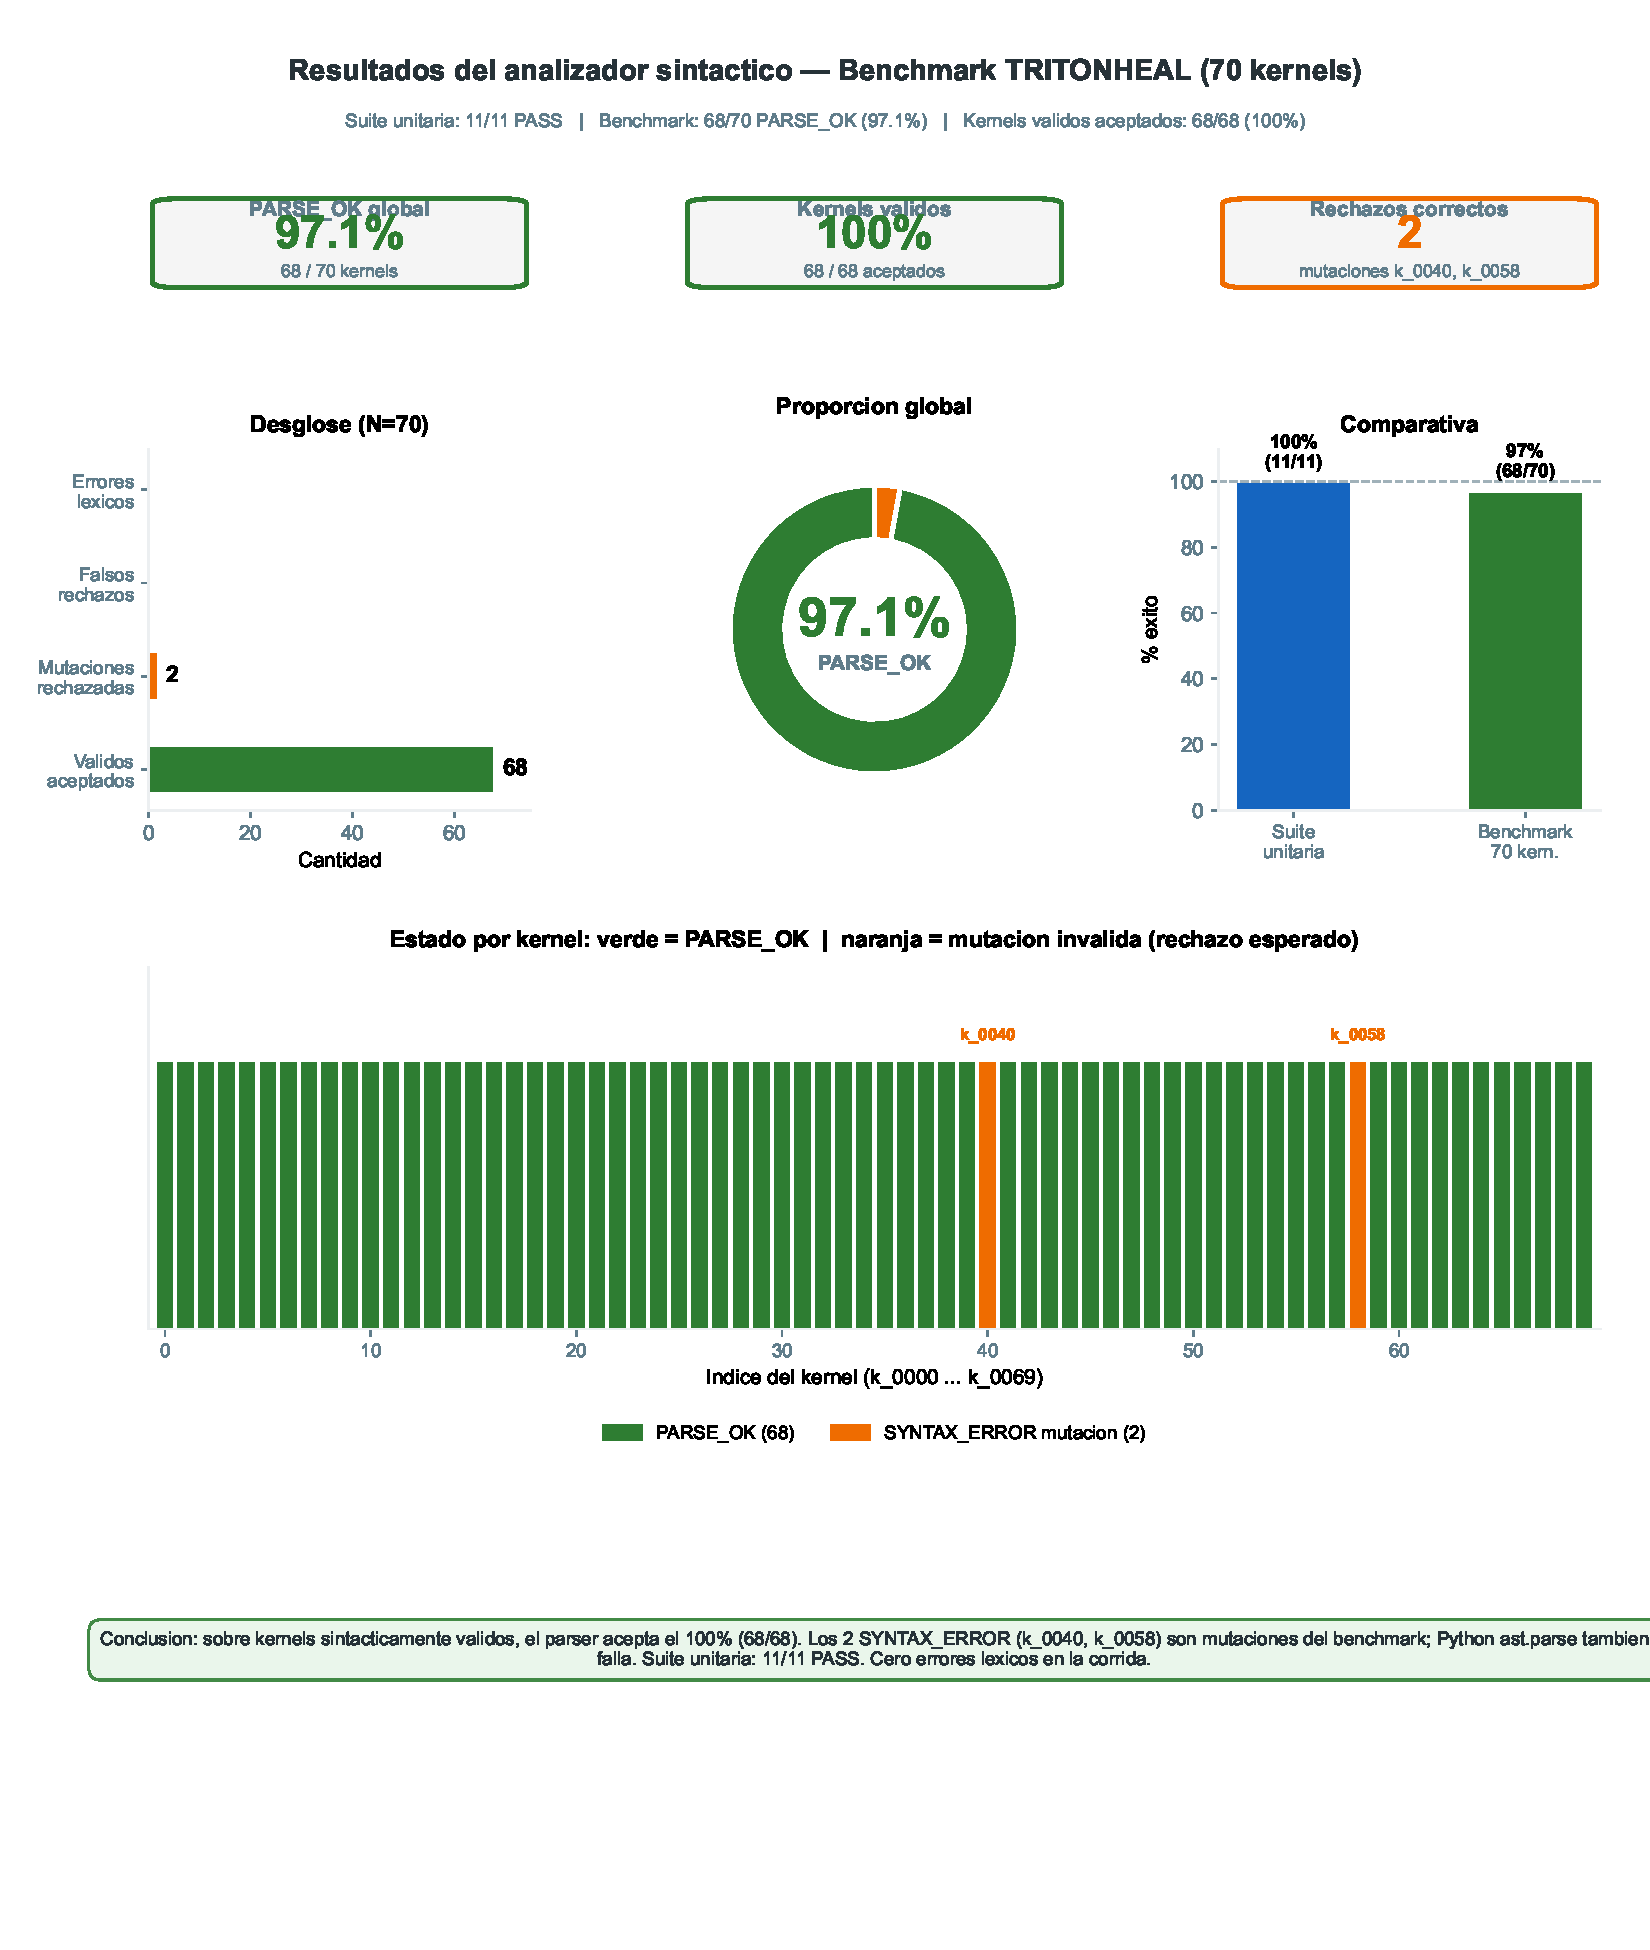
\includegraphics[width=\linewidth]{benchmark_parse_results.pdf}
\caption{%
\textbf{Resultados del analizador sintáctico.} Panel superior: indicadores clave. Centro izquierda: desglose (68 válidos aceptados, 2 mutaciones rechazadas, 0 falsos rechazos). Centro derecha: 97.1\% PARSE\_OK global. Inferior: mapa de los 70 kernels (\texttt{k\_0000}--\texttt{k\_0069}); verde = éxito, naranja = mutación inválida (\texttt{k\_0040}, \texttt{k\_0058}).
}
\label{fig:benchmark70}
\end{figure}

\subsection{Detalle de los 2 rechazos (comportamiento esperado)}
\begin{table}[H]
\centering
\caption{Kernels rechazados: mutaciones inválidas del benchmark.}
\label{tab:rechazos}
\begin{tabular}{@{}llp{6.5cm}@{}}
\toprule
\textbf{Kernel} & \textbf{Verificación Python} & \textbf{Motivo del rechazo} \\
\midrule
\texttt{k\_0040.tri} & \texttt{ast.parse} falla & \texttt{tl.store(out\_ptr + offs) \& ...} --- paréntesis inválido. \\
\texttt{k\_0058.tri} & \texttt{ast.parse} falla & \texttt{tl.store(...), mask=...)} --- coma mal ubicada. \\
\bottomrule
\end{tabular}
\end{table}

Estos rechazos demuestran que el parser \textbf{detecta errores sintácticos} con el mensaje \texttt{SYNTAX\_ERROR}, cumpliendo el entregable de mensajes de error del documento de evaluación.

%------------------------------------------------------------------------------
\subsection{Modelo de pruebas}
\textbf{Verificación}: ¿se construyó el producto correctamente? --- compila, ejecuta, mensajes coherentes.\\
\textbf{Validación}: ¿es el producto correcto? --- acepta Triton válido y rechaza inválido.

\subsection{Suite unitaria (\texttt{make test})}
\begin{table}[H]
\centering
\caption{Casos de prueba del equipo (11 ejecuciones).}
\begin{tabular}{@{}llc@{}}
\toprule
ID & Descripción & Resultado \\
\midrule
V1--V3 & \texttt{ejemplo\_1..3.tri} (reporte léxico) & PASS \\
V4--V5 & Kernels Triton mínimos & PASS \\
I1--I5 & Sintaxis inválida deliberada & SYNTAX\_ERROR \\
I6 & Identificador con \texttt{BAD\_ID} (\texttt{x\$}) & LEXICAL\_ERROR \\
L1 & Modo \texttt{-t} tokens & PASS \\
\midrule
\multicolumn{2}{l}{\textbf{Total PASS}} &
\IfFileExists{data/parser_pass.tex}{\input{data/parser_pass.tex}}{12} / \IfFileExists{data/parser_total.tex}{\input{data/parser_total.tex}}{12} \\
\bottomrule
\end{tabular}
\end{table}

\subsection{Evidencia: salida exitosa (\texttt{ejemplo\_1.tri})}
\IfFileExists{../results/parser/valid_ejemplo_1.tri.log}{%
\lstinputlisting[caption={Log de exito (\texttt{ejemplo\_1.tri}, extracto).}, basicstyle=\ttfamily\scriptsize, lastline=22]{../results/parser/valid_ejemplo_1.tri.log}
}{}

\subsection{Evidencia: error sintáctico (\texttt{def\_sin\_dos\_puntos.tri})}
\IfFileExists{../results/parser/invalid_def_sin_dos_puntos.tri.log}{%
\lstinputlisting[caption={Rechazo sintáctico esperado (suite unitaria).}, basicstyle=\ttfamily\scriptsize, lastline=5]{../results/parser/invalid_def_sin_dos_puntos.tri.log}
}{}

\subsection{Evidencia: error léxico \texttt{BAD\_ID} (I6)}
\IfFileExists{../results/parser/invalid_identificador_caracter_invalido.tri.log}{%
\lstinputlisting[caption={Rechazo por identificador con \texttt{\$} (regla \texttt{BAD\_ID}, alineada con Analizador-lexico).}, basicstyle=\ttfamily\scriptsize, lastline=3]{../results/parser/invalid_identificador_caracter_invalido.tri.log}
}{}

\subsection{Reproducibilidad}
\label{sub:reproducibilidad}

\noindent Todo el material para reproducir el proyecto en una \textbf{PC nueva} está en el repositorio público (sin dependencias externas de otros repos):

\begin{itemize}
  \item Repositorio: \url{https://github.com/G4ndhiV/Analizador-sint-ctico}
  \item Kernels de prueba: \path{benchmark/kernels/} (70 archivos \texttt{k\_*.tri})
  \item Fixtures léxicos: \path{tests/fixtures/lexico/}
  \item CFG documentada: \path{report/cfg/triton_cfg.bnf}
  \item Resultados de referencia: \path{results/parser/}, \path{results/benchmark/}
  \item Informe PDF: \path{deliverables/Informe_Analizador_Sintactico_Equipo11.pdf}
\end{itemize}

\subsubsection{Prerrequisitos}
\begin{table}[H]
\centering
\caption{Software necesario para reproducir compilación, pruebas, gráfica e informe.}
\label{tab:repro-deps}
\small
\begin{tabular}{@{}llp{5.8cm}@{}}
\toprule
\textbf{Herramienta} & \textbf{Obligatorio} & \textbf{Instalación típica} \\
\midrule
\texttt{git} & Sí & Clonar el repositorio \\
\texttt{cc} (GCC/Clang) & Sí & Xcode CLT (macOS) o \texttt{build-essential} (Linux) \\
Bison & Sí & \texttt{brew install bison} / \texttt{apt install bison} \\
Flex & Sí & \texttt{brew install flex} / \texttt{apt install flex} \\
Python~3 + \texttt{venv} & Sí (gráfica) & \texttt{python3 -m venv .venv}; \texttt{pip install -r requirements.txt} \\
Tectonic o \texttt{latexmk} & Solo para \texttt{make pdf} & \texttt{brew install tectonic} \\
\bottomrule
\end{tabular}
\end{table}

Verificación rápida: \texttt{make check-deps} (objetivo del \texttt{Makefile} raíz).

\subsubsection{Pasos desde cero (PC nueva)}
\begin{enumerate}
  \item \textbf{Clonar:}
\begin{verbatim}
git clone https://github.com/G4ndhiV/Analizador-sint-ctico.git
cd Analizador-sint-ctico
\end{verbatim}
  \item \textbf{Comprobar dependencias (opcional):} \texttt{make check-deps}
  \item \textbf{Compilar:} \texttt{make build} $\rightarrow$ ejecutable \texttt{build/triton\_parser}
  \item \textbf{Suite unitaria:} \texttt{make test} $\rightarrow$ \textbf{12/12 PASS}; logs en \texttt{results/parser/}
  \item \textbf{Benchmark 70 kernels:} \texttt{make benchmark} $\rightarrow$ \texttt{results/benchmark/summary.json}
  \item \textbf{Gráfica:} \texttt{make figures} $\rightarrow$ \texttt{figures/benchmark\_parse\_results.pdf}
  \item \textbf{Informe PDF:} \texttt{make pdf} $\rightarrow$ ver ruta en \path{deliverables/Informe_Analizador_Sintactico_Equipo11.pdf}
\end{enumerate}

\subsubsection{Comando único (regeneración completa)}
\begin{verbatim}
make clean build test benchmark figures pdf
\end{verbatim}

\subsubsection{Salidas verificables}
\begin{itemize}
  \item \path{results/parser/summary.json}: \texttt{"pass": 12}, \texttt{"total": 12}.
  \item \path{results/benchmark/summary.json}: \texttt{parse\_ok}: 68, \texttt{total}: 70.
  \item \path{figures/benchmark_parse_results.pdf} y \path{figures/benchmark_parse_results.png}.
  \item PDF del informe en \path{deliverables/} (Apéndice~A: CFG de 91 producciones).
\end{itemize}

\subsubsection{Consulta sin recompilar}
Basta con clonar el repositorio y abrir el PDF en \path{deliverables/} y los archivos \path{results/parser/summary.json} y \path{results/benchmark/summary.json}.

\subsubsection{Notas por sistema operativo}
\begin{itemize}
  \item \textbf{macOS:} instalar \texttt{bison} y \texttt{flex} con Homebrew; el \texttt{Makefile} enlaza la librería Flex de Homebrew.
  \item \textbf{Linux:} usar \texttt{bison} y \texttt{flex} del sistema; enlace con \texttt{-lfl}.
  \item \textbf{\texttt{BAD\_ID}:} reglas en \path{lexer/lexico_equipo_11_scanner.l} (repo léxico: \url{https://github.com/G4ndhiV/Analizador-lexico}); prueba I6 en \path{tests/invalid/identificador_caracter_invalido.tri}.
\end{itemize}

Guía extendida: \path{README.md} en la raíz del repositorio.

\section{Plan de Trabajo}

\begin{table}[H]
\centering
\caption{Cronograma de la fase sintáctica (Equipo 11).}
\begin{tabular}{@{}cll@{}}
\toprule
Fase & Actividad & Entregable \\
\midrule
1 & Revisión tokens léxicos y kernels TRITONHEAL & Inventario de requisitos \\
2 & Diseño CFG + resolución indentación & Documento de análisis \\
3 & Especificación yacc + symtab & \texttt{parser.y}, \texttt{symtab.c} \\
4 & Integración Flex--yacc + driver & \texttt{triton\_parser} \\
5 & Suite de pruebas + benchmark 70 & \texttt{tests/}, \texttt{results/} \\
6 & Reporte IEEE-830 + gráfica & PDF final \\
\bottomrule
\end{tabular}
\end{table}

\subsection{Distribución de responsabilidades}
\begin{itemize}
  \item Gramática y yacc: análisis conjunto del equipo, implementación en \texttt{parser.y}.
  \item Lexer integrado: extensión de \texttt{lexico\_equipo\_11\_scanner.l}.
  \item Pruebas y benchmark: scripts \texttt{run\_tests.sh}, \texttt{run\_benchmark\_kernels.sh}.
  \item Reporte y figuras: \LaTeX{} + \texttt{plot\_benchmark\_results.py}.
\end{itemize}

\appendix
\section{Gramática libre de contexto completa}
\label{ap:cfg-completa}

Esta sección presenta la \textbf{CFG completa} del subconjunto de Python/Triton implementado en \texttt{parser/parser.y}. Cada producción corresponde a una regla yacc sin las acciones semánticas en C. Las producciones vacías del analizador se denotan como \texttt{epsilon} ($\varepsilon$).

\textbf{Convenciones:}
\begin{itemize}
  \item \texttt{ID}, \texttt{INT}, \texttt{FLOAT}, \texttt{STRING} $\equiv$ \texttt{TOKEN\_IDENTIFIER}, \texttt{TOKEN\_INTEGER}, \texttt{TOKEN\_FLOAT}, \texttt{TOKEN\_STRING}.
  \item \texttt{OP} $\equiv$ \texttt{TOKEN\_OPERATOR} (p.\,ej.\ lexema \texttt{=}, \texttt{+}, \texttt{*}).
  \item \texttt{DELIM} $\equiv$ \texttt{TOKEN\_DELIMITER} cuando el léxico clasifica un símbolo como delimitador en expresiones.
  \item \texttt{NEWLINE}, \texttt{INDENT}, \texttt{DEDENT} $\equiv$ tokens 950, 910 y 911 (sintéticos desde \texttt{WS\_COUNT}).
  \item \texttt{KW\_*} son terminales de palabra reservada (\texttt{def}, \texttt{if}, \texttt{import}, \texttt{None}, etc.).
  \item Paréntesis, corchetes, dos puntos, coma y punto son literales en la gramática yacc.
\end{itemize}

\subsection{Terminales del analizador}
\begin{table}[H]
\centering
\caption{Conjunto de terminales (yacc / reporte léxico).}
\label{tab:terminales-cfg}
\small
\begin{tabular}{@{}clp{6.8cm}@{}}
\toprule
\textbf{Símbolo} & \textbf{ID} & \textbf{Descripción} \\
\midrule
\texttt{ID} & 100 & Identificadores \\
\texttt{KW\_*} & 101 & Palabras reservadas (\texttt{def}, \texttt{if}, \texttt{for}, \ldots) \\
\texttt{INT} & 200 & Enteros \\
\texttt{FLOAT} & 300 & Flotantes \\
\texttt{STRING} & 400 & Cadenas \\
\texttt{OP} & 500 & Operadores \\
\texttt{DELIM} & 600 & Delimitadores léxicos \\
\texttt{COMMENT} & 700 & Comentarios (descartados en parseo) \\
\texttt{INDENT} & 910 & Inicio de bloque indentado \\
\texttt{DEDENT} & 911 & Fin de bloque indentado \\
\texttt{NEWLINE} & 950 & Fin de línea \\
\texttt{'@'}, \texttt{'.'}, \texttt{'('}, \texttt{')'}, \texttt{'['}, \texttt{']'}, \texttt{':'}, \texttt{','} & --- & Literales en reglas yacc \\
\bottomrule
\end{tabular}
\end{table}

\subsection{Precedencia y asociatividad (yacc)}
Las ambigüedades de expresiones y de la regla \texttt{if}--\texttt{else} se resuelven con las directivas de \texttt{parser.y} (de menor a mayor precedencia en la pila):

\begin{table}[H]
\centering
\caption{Orden de precedencia (\texttt{\%left} / \texttt{\%nonassoc}).}
\label{tab:precedencia-cfg}
\begin{tabular}{@{}lll@{}}
\toprule
\textbf{Precedencia} & \textbf{Asociatividad} & \textbf{Terminales} \\
\midrule
1 (más baja) & izquierda & \texttt{NEWLINE} \\
2 & izquierda & \texttt{KW\_OR} \\
3 & izquierda & \texttt{KW\_AND} \\
4 & no asoc. & \texttt{KW\_NOT} \\
5 & izquierda & \texttt{OP}, \texttt{DELIM} (en \texttt{expr}) \\
6 & no asoc. & \texttt{KW\_ELIF} \\
7 (más alta) & no asoc. & \texttt{KW\_ELSE} \\
\bottomrule
\end{tabular}
\end{table}

\subsection{Producciones (33 no terminales)}
El listado siguiente agrupa las \textbf{33 reglas no terminales} de la implementación: \texttt{program}, \texttt{opt\_newlines}, \texttt{top\_block}, \texttt{top\_line}, \texttt{stmt}, \texttt{import\_stmt}, \texttt{import\_name}, \texttt{opt\_as}, \texttt{triton\_decorator}, \texttt{opt\_triton\_decorator}, \texttt{def\_stmt}, \texttt{param\_list\_opt}, \texttt{param\_list}, \texttt{param}, \texttt{suite}, \texttt{block\_body}, \texttt{block\_stmt}, \texttt{simple\_stmt}, \texttt{assign\_stmt}, \texttt{if\_stmt}, \texttt{elif\_parts}, \texttt{else\_part}, \texttt{while\_stmt}, \texttt{for\_stmt}, \texttt{return\_stmt}, \texttt{pass\_stmt}, \texttt{expr\_stmt}, \texttt{expr}, \texttt{opt\_expr}, \texttt{subscript\_list}, \texttt{subscript}, \texttt{unary\_expr}, \texttt{member\_chain}, \texttt{call\_expr}, \texttt{arg\_list\_opt}, \texttt{arg\_list}, \texttt{arg}.

\lstinputlisting[
  basicstyle=\ttfamily\scriptsize,
  breaklines=true,
  frame=single,
  numbers=left,
  numberstyle=\tiny,
  caption={CFG completa del lenguaje \texttt{.tri} (archivo \texttt{report/cfg/triton\_cfg.bnf}).},
  label={lst:cfg-completa}
]{cfg/triton_cfg.bnf}

\subsection{Trazabilidad CFG $\rightarrow$ implementación}
La gramática de este apéndice es la referencia formal del entregable; la implementación ejecutable está en \texttt{parser/parser.y} (reglas entre las marcas \texttt{\%\%}). Cualquier cambio en yacc debe reflejarse en \texttt{triton\_cfg.bnf} para mantener consistencia documental.

\section{Referencias}

\begin{enumerate}
  \item R. J. Castelló, ``Chapter 3: Syntax Analysis, Part I --- Grammar Processing,'' \textit{Module \#3: Compilers} (TC3002B, Advanced Applications Development), notas de curso, ITESM, s.\,f.
  \item R. J. Castelló, ``Chapter 2: Lexical Analysis,'' \textit{Module \#3: Compilers} (TC3002B), notas de curso, ITESM, s.\,f.
  \item Equipo 11, \textit{Analizador Léxico --- Triton GPU Kernel}, reporte TC3002B, entrega mayo 2026.
  \item Salvador Hinojosa, \textit{Evaluation Metrics Syntax Analyzer GDL Triton}, TC3002B, documento de evaluación, 2026.
  \item OpenAI, \textit{Triton: Open-Source GPU Programming}, [en línea]; disponible en \url{https://triton-lang.org}; Internet.
  \item A. V. Aho, M. S. Lam, R. Sethi y J. D. Ullman, \textit{Compilers: Principles, Techniques, and Tools}, 2nd ed., Addison-Wesley, 2007.
  \item Proyecto TRITONHEAL, benchmark de 70 kernels \texttt{k\_*.tri}, repositorio de referencia del Equipo~11, 2026.
\end{enumerate}


\end{document}
